\documentclass[11pt]{article}
\usepackage{graphicx}
\usepackage{geometry}
\usepackage{graphicx}
\usepackage{amsmath}
\usepackage{siunitx}
\usepackage{subcaption}
\usepackage{flafter}
\usepackage{float}
\usepackage{tabularx}
\usepackage[section]{placeins}
 \geometry{
 a4paper,
 total={170mm,257mm},
 left=2cm,
 top=2cm,
 right= 2cm,
 bottom = 2cm
}
\usepackage[T1]{fontenc}
\usepackage{mathptmx}
\usepackage{amsmath}
\usepackage{siunitx}
\usepackage{float}
\usepackage{setspace}
\usepackage[style=apa, backend=biber]{biblatex}
\title{\textbf{Subject: Psychology} \\[1ex]\large RQ: How does priming affect decision-making by speed estimation?}
\author{}
\date{\today}
\addbibresource{mybibliography.bib}
\doublespacing
%\setlength\bibhang{0pt}
\begin{document}
\date{Word Count:1869\\Personal Code: lch068  | Co-researcher Code: lch077  \\ \today }
\maketitle
\newpage
\tableofcontents
\iffalse
\section{Abstract}
The aim of this experiment was to investigate if priming  would affect decision-making by speed estimation. The hypothesis predicted that priming with aggressive words would lead to a higher speed estimation by the participants. This study was based of the study done by Loftus and Palmer~\autocite{loftus1974}, 
where the aforementioned hypothesis was proven to be true. The DV was the speed estimation of a car right before it crashed, and the IV was the choice of 3 words that had different semantics attached to them.
An opportunity sample of 38 participants $N=38$ participated. The participants were shown a video from a car crash. This video was part of the list of videos that the original study used. The participants where divided into 3 groups and a questionnaire was given to each subject.
The questionnaire contained 3 filler questions and 1 significant question. For each group, the only difference in the questionnaire was the use of priming word: Smashed, Collided or Bumped. The significant question asked the subject to estimate the speed of the car.

Using a One Way ANOVA test, the results were statistically significant at $p<0.001$, so the hypothesis that priming with words which are semantically aggressive would lead the subject to estimate a higher speed of the car. This result was in compliance with the original study. 

\fi
\section{Introduction}
When a memory is created, it is not stored like a file on a smartphone that can be played back, instead a memory construction process takes place, which works by encoding different senses (Iconic, Haptic, Echoic, Gustatory and Olfactory), together with emotions and semantics.
When recalling an event, these memories are reconstructed from the fragments of information that were previously encoded~\autocite{Stark2010}.

But sometimes during the reconstruction of memories, the brain takes cognitive shortcuts to achieve efficiency, which leads to false memories. The false memories can be created before a recall or during recall of memories. The false memories created during recall use heuristics to achieve cognitive efficiency. Heuristics, first introduced by Daniel Kahneman~\autocite{Kahneman1974} are decision making rules that are used by people to efficiently make decisions, that is using minimal cognitive effort.
Minimal cognitive effort results in not only faster decision-making but also conservation of energy to be utilized in other areas of the body. But, heuristics are the prime reason for the formation of biases in decision making.
False memories created before the process of reconstructive memories are likely due to the misinformation effect. The misinformation effect is a cause of false memories that occurs due to the introduction of misleading information. This misleading information incorporates itself into the memory of a particular event in the past.
Elizabeth Loftus studied false memories in great detail and in the study~\autocite{loftus1974}, she focused on the biases in decision-making that stems from false memories. The study contained 2 experiments and the aim of both experiments was to study the effects of use the misinformation effect by using linguistic characteristics to induce false reconstructive memory and study the biases in decision making.
The use of specific linguistic characteristics to evoke certain semantics is based on the theory of priming.
Priming occurs when an individual is exposed to certain stimuli which subconsciously affects their response to another stimuli. According to a study conducted by Carmichael, that recalling of certain memories may be determined by the nature of the words that are presented to the subjects during the recalling process.~\autocite{carmichael1932}.
This conclusion was used to form the methodology for the study~\autocite{loftus1974}. 



It is important to study this effect as the formation of false memories can lead to false eyewitness testimonies, which results in false imprisonment of innocent people. It is important to study this effect to understand how to avoid misinformation and view an event from an objective point of view.
This research is a replication of the first experiment of~\autocite{loftus1974} with the primary goal of investigating the effects of priming. 
The aim of this experiment was to investigate if priming would affect decision making by speed estimation. This experiment aims to replicate the study~\autocite{loftus1974}, to establish
reliability and further the understanding of false memories.
Based on the results of the original experiment a direct hypothesis was chosen.
\\\\
\textbf{Experimental Hypothesis $H_1$:} Priming the participants with words that are perceived to be more violent were more likely to estimate significantly higher speeds of the car shown in the video.
\\
\textbf{Null Hypothesis $H_0$:} Priming the participants with words that are perceived to be more violent would not affect the estimation of speed of the car shown in the video.



\section{Methodology}

\textbf{Design:} \newline
The independent sample design was chosen since assigning one subject to multiple conditions risked a chance of biased results due to priming multiple times. This research utilized a lab experimental method to establish cause and effect. 
This allowed us to control the experimental conditions, such that performing the experiment on different subjects at different times would still yield similar results.
Ethical considerations were thoroughly followed. The participants were briefed before the experiment and debriefed after it. They were informed that they have all the right to withdraw from the experiment and are entitled to the results of the experiment.
The consent of each participant was taken through the T\&C of the school, where the school has the right to survey the student as long as they were not harmed physically or psychologically. Additionally, they were asked to give a verbal consent and were in no circumstances obligated to participate in the experiment.
No participants withdrew from the experiment. \newline
\textbf{Variables:}\newline
\textbf{Independent Variable}: Verbs\newline 
\textbf{Independent Variable Operationalization}: Categorizing different groups to each verb by perceived intensity\\
\textbf{Dependent Variable}: Speed estimation\newline
\textbf{Dependent Variable Operationalization}: A questionnaire \\
\textbf{Controlled Variable}: 
\begin{itemize}
  \item \underbar{Age}: A large delta in age could result in different justification of speed estimations. People aged 30\-40 years are more likely to be experienced in driving than from ages 16\-18, due to differently formed schemas. Hence, limiting the range of ages, allows the cause effect to be observed regardless of vastly different personal experience.
  \item \underbar{Experimental Conditions:} All subjects were tested in the same room under the same conditions. Doing so otherwise, could potentially affect the priming and recalling process. Subjecting the participants to the same conditions will allow for a similar cognitive process taking place.
\end{itemize}
\textbf{Participants:}\newline
The participants were found using ``Opportunity sampling'' as it was the most convenient and time efficient. The target populations were the IB students at EKOLA International School with a fluency in English.
The participants who consented to participate were taken to an empty classroom and were seated appropriately. This experiment was performed on twice on different groups in similar experimental conditions.
The sample consisted of 17 males and 21 females ($N=38$), between the ages 15\hyphen18 years ($\leq a \leq 18$ years, $\overline{a}=16.7$, $\sigma_a=0.8$ years, $\tilde{a}=17$ years).\\
The participants were divided into 3 groups called ``Smashed'', ``Collided'' and ``Bumped''.
\\
This experiment was performed twice on 2 different sets of groups in order to gather appropriate amount of samples $N$. The group ``Smashed'' consisted of 7 males and 6 females ($N_s=13$). ``Collided'' consisted of 7 males and 7 Females ($N_c=14$) and ``Bumped'' consisted of 4 males and 7 females ($N_b=11$).\\\\
\textbf{Materials Used:}\newline
\begin{itemize}
  \item Briefing and Debriefing instructions \textit{(figures~\ref{fig:briefing} and~\ref{fig:debriefing})}
  \item Multiple copies of the questionnaire for 3 groups. \textit{(figures~\ref{ques:smashed},~\ref{ques:collided} and~\ref{ques:bumped})}
  \item Digital whiteboard
  \item 10s video of a car crash.
\end{itemize}
\textbf{Procedure:}\newline
Each participant was firstly briefed about the experiment. The words for briefing \textit{(figure~\ref{fig:briefing})} were carefully chosen as to reveal minimal information about the experiment and reduce risk of biased results. 
The participants were shown a 10-second video of a car crash. The participant then turned their questionnaires \textit{(figures~\ref{ques:smashed},~\ref{ques:collided} and~\ref{ques:bumped}) }from face up and answered them. After everyone finished writing, the questionnaires were collected
and the participants were debriefed. Each participant were randomly divided into 3 separate groups (``Smashed'', ``Collided'', ``Bumped'') and the questionnaires they received were different by only a word. This different word was the same as their group.
As in the group ``Smashed'', received the questionnaire with the word ``Smashed'' \textit{(figure~\ref{ques:smashed})}.
The question with the different word was at the end as it was the critical question. The critical question asked the subject to estimate the speed of the focus car during the crash.
All questions above were to distract the subject from the significant question and verify if the answer was valid, meaning the subject answered them with full seriousness.\\\\

The raw data~(\textit{Table~\ref{tab:rawData}}) was collected and manually inputted into Jamovi~\cite{6}. Then using Jamovi and its built-in statistical libraries~\cite{7} and~\cite{8}, One-Way Anova test was performed to get the descriptive and inferential statistics. 
\section{Results}
\subsection{Descriptive statistics}
This study collected interval data and hence, the mean and standard deviation were chosen as descriptive statistics. \textit{(Table~\ref{tab:desc})} shows the descriptive statistics of different groups' speed estimation.
In the table (\textit{Table~\ref{tab:desc}}) it can be seen that on average, subjects primed with the verb ``Smashed'', estimated higher speeds ($\bar{S}=99.2km/s$) as compared to ``Collided'' ($\bar{C}=62.4km/h$)  and ``Bumped'' ($\bar{B}=36.1km/h$), with the latter having the lowest speed estimation
The Standard Deviation ($SD$) shows that the results were dispersed fairly wide, with $SD_s=22.9km/h$, $SD_c=16.9km/h$, $SD_b=12.0km/h$. The mean and SD of different groups are represented graphically in \textit{(Figure~\ref{fig:mean})} and \textit{(Figure~\ref{fig:SD})}


\begin{table}[!ht]
  \centering
  \caption{ ~\\Descriptive data}
  \begin{tabular}{|l|l|l|l|l|}
  \hline
      \textbf{Groups} & \textbf{N} & \textbf{$Mean [km/h]$} & \textbf{$SD [km/h]$} & \textbf{$SE [km/h]$} \\ \hline
      \textbf{Smashed} & 13 & 99.2 & 22.9 & 6.35 \\ \hline
      \textbf{Collided} & 14 & 62.4 & 16.9 & 4.51 \\ \hline
      \textbf{Bumped} & 11 & 36.1 & 12.0 & 3.63 \\ \hline
  \end{tabular}
~\label{tab:desc}
\end{table}

\begin{figure}[H]
  \caption{ ~\\Bar Graph of Average estimations ($\bar{S},\bar{C}, \bar{B}$) for each group} 
  \centering 
  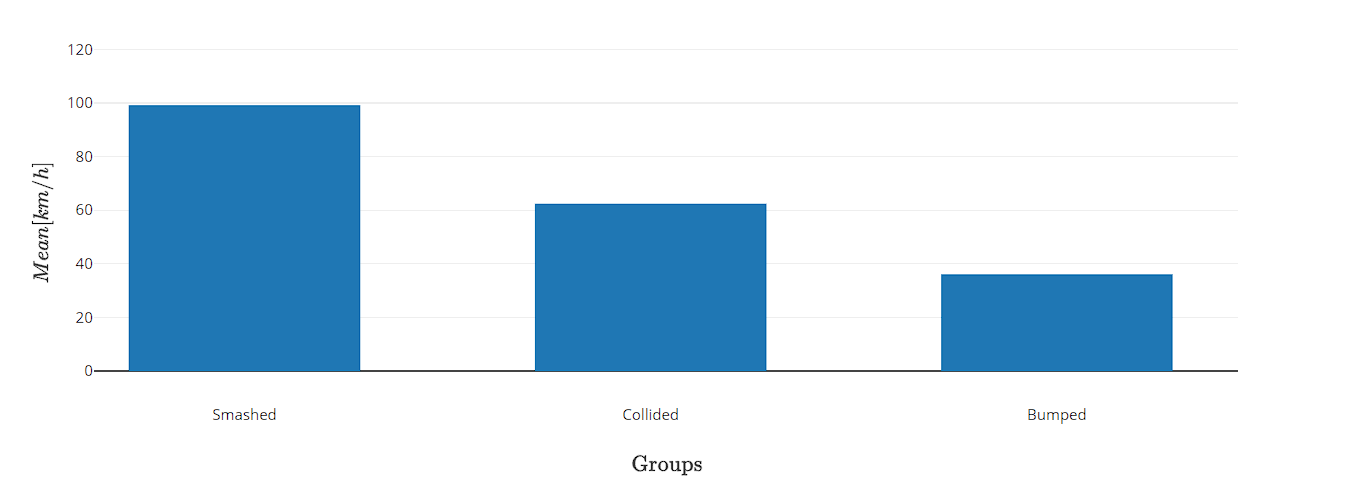
\includegraphics[width=\textwidth]{mean.png}
~\label{fig:mean}
\end{figure}

\begin{figure}[H]
  \caption{ ~\\Bar Graph of Standard Deviation ($SD_s, SD_c, SD_b$) for each group} 
  \centering 
  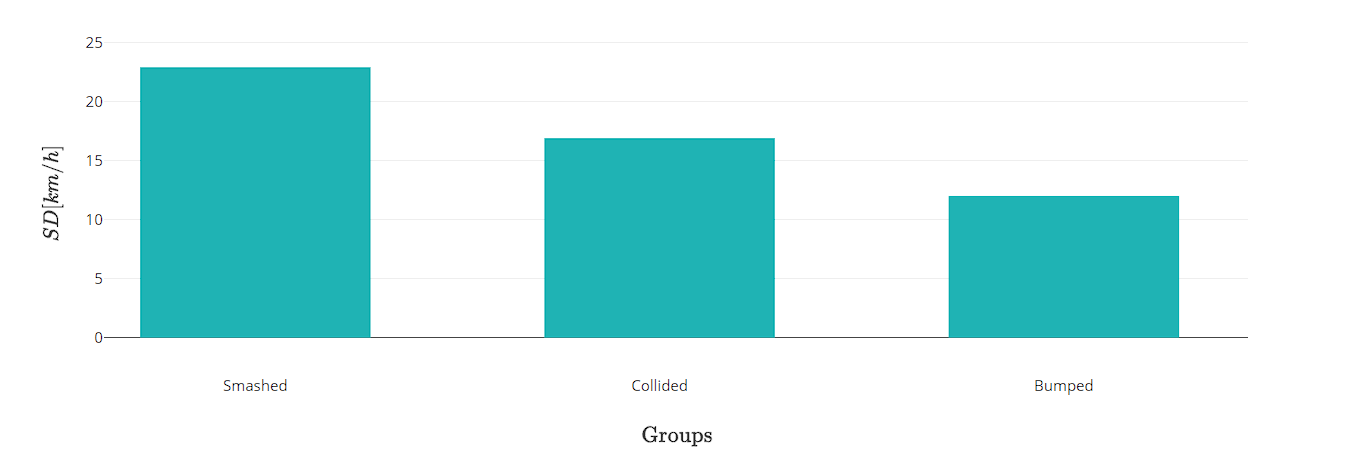
\includegraphics[width=\textwidth]{SD.png}
~\label{fig:SD}
\end{figure}


%\bibliographystyle{apalike}
%bibliography{mybibliography.bib}
\subsection{Inferential statistics}
A One Way ANOVA test was used since the experiment tested a difference between 3 groups. Using a Statistical tool, Fisher's Variance $F(2,35)=37.2$, and $p<0.001$ (statistical significance)  were calculated.
The low statistical significance means that the difference in the speed estimation between groups were significant enough for the null hypothesis can be rejected and the experimental hypothesis can be accepted.
\\
The results from the descriptive and inferential statistics show that similar words with different semantics, do lead to a bias in decision making which was reflected by the estimation of speed.
\section{Conclusion}
This experiment showed that priming the subjects lead to the misinformation effect which resulted in a biased decision-making. This conclusion was reflected by the subject in group ``Smashed'', estimating a higher speed than groups ``Bumped'' and ``Contacted''.
On participant specifically stated in the answer to the significant question that they did not see the car crash as they were distracted. Yet this subject, from group ``Smashed'' estimated a relatively high car speed~\textit{figure~\ref{fig:outlier}}
\section{Evaluation}
Despite the conclusions being consistent with the original study, this study conducted resulted in several strengths and limitations. 
\\\\
\textbf{Firstly}, this study uses a sample consisting of international students. This allowed for a cause effect to be established across multiple cultures. Additionally, everyone in the sample
had a fluency in English language which was necessary for the priming effect to work. This established the external validity of this experiment.
\\
\textbf{Secondly}, a high internal validity was established the use of lab experimental method which helped factor out the controlled variables hence assuring that every subject participated in the experiment in very similar environment\\
\\
\textbf{Moreover}, The study used independent measure design, which contributed to the credibility of the experiment. The original study used repeated measures, but it was disregarded for this study as it would have resulted in the subject already familiarized
with the questionnaire when redoing the experiment under different conditions. While the use of matched pair design would make it difficult to isolate the independent variable due to other factors such as age, gender and race needing to be accounted for.\\
\\
\textbf{Lastly}, ethical concerns were also attended to. Briefing and debriefing the participants allowed the study to be overt and ethical. Each participant had the right to withdraw anytime they wished to until submission since the form couldn't be traced back.
\\\\
Albeit the strengths, the study has certain limitations also, that could be further improved upon the replication of this experiment. 
\\\\
\textbf{Firstly}, the sample size was relatively small, and restricted to 3rd year high school students. Due to participants all attending a private international school, they belong to a relatively high socio-economic status.
This decreases the generalizability of the experiment, as they do not represent the whole of population.
%\textbf{Firstly}, the average speed estimate in this study was about $58km/h$ higher than the orignal study for group ``Smashed'', while for ``Collided'' the mean estimation was higher by about $30km/h$ than the orignal study~\cite{loftus1974}. The mean estimate for the group
%``Bumped'' was relatively close to the orignal study with the difference being $2km/h$ higher in this study. This difference can be explained by the theory that the semantics of certain words have changed over time, and words ``Smashed'' and ``Collided'' have a much more intense effect.
\\
\textbf{Another} major limitation was the flaw in the questionnaire with the critical question ``What was the speed of the focus car?'', these 3 participants' answer to with ``I do not know''. An improvement to this would be to phrase the 
critical question as ``Estimate the speed of the focus car:?''
\\
The \textbf{third} limitation of this experiment is, that one cannot be certain if a memory was constructed of the car speed or simply the estimation was biased due to use of language. This experiment concludes that it might be a combination of both
where the use of semantically heavy language influenced, influenced the memory reconstruction. This negatively affects the internal validity as doubts about an isolated cause effect still exist.
\\
\textbf{Lastly}, the use of experimental methods introduces artificiality. This decreases the applicability of the findings as the subjects may or may not perform differently in a naturalistic environment. 


\printbibliography{}
\section*{Appendix}
\begin{table}[!ht]
  \centering
  \caption{ ~\\Raw data collected from the experiment processed in~\cite{6}}
  \begin{tabular}{|l|l|l|l|l|}
  \hline
      \textbf{N} & \textbf{Group} & \textbf{Speed Estimated [km/h]} & \textbf{Gender [F/M]} & \textbf{Age} \\ \hline
      1 & "Collided" & 80 & "F" & 17 \\ \hline
      2 & "Collided" & 95 & "F" & 17 \\ \hline
      3 & "Collided" & 80 & "M" & 18 \\ \hline
      4 & "Collided" & 60 & "F" & 17 \\ \hline
      5 & "Collided" & 41 & "F" & 17 \\ \hline
      6 & "Collided" & 67 & "M" & 17 \\ \hline
      7 & "Collided" & 60 & "F" & 17 \\ \hline
      8 & "Collided" & 35 & "M" & 16 \\ \hline
      9 & "Collided" & 50 & "F" & 15 \\ \hline
      10 & "Collided" & 50 & "F" & 16 \\ \hline
      11 & "Collided" & 50 & "M" & 15 \\ \hline
      12 & "Collided" & 65 & "M" & 18 \\ \hline
      13 & "Collided" & 60 & "M" & 17 \\ \hline
      14 & "Collided" & 80 & "F" & 17 \\ \hline
      15 & "Bumped" & 40 & "F" & 17 \\ \hline
      16 & "Bumped" & 30 & "M" & 17 \\ \hline
      17 & "Bumped" & 35 & "F" & 17 \\ \hline
      18 & "Bumped" & 27 & "F" & 17 \\ \hline
      19 & "Bumped" & 40 & "F" & 17 \\ \hline
      20 & "Bumped" & 40 & "M" & 18 \\ \hline
      21 & "Bumped" & 60 & "F" & 18 \\ \hline
      22 & "Bumped" & 15 & "F" & 17 \\ \hline
      23 & "Bumped" & 30 & "M" & 16 \\ \hline
      24 & "Bumped" & 30 & "M" & 17 \\ \hline
      25 & "Bumped" & 50 & "F" & 16 \\ \hline
      26 & "Smashed" & 100 & "F" & 17 \\ \hline
      27 & "Smashed" & 60 & "F" & 17 \\ \hline
      28 & "Smashed" & 120 & "M" & 17 \\ \hline
      29 & "Smashed" & 100 & "M" & 17 \\ \hline
      30 & "Smashed" & 100 & "M" & 17 \\ \hline
      31 & "Smashed" & 100 & "M" & 16 \\ \hline
      32 & "Smashed" & 80 & "M" & 16 \\ \hline
      33 & "Smashed" & 70 & "F" & 17 \\ \hline
      34 & "Smashed" & 100 & "M" & 17 \\ \hline
      35 & "Smashed" & 120 & "F" & 17 \\ \hline
      36 & "Smashed" & 100 & "F" & 16 \\ \hline
      37 & "Smashed" & 150 & "M" & 15 \\ \hline
      38 & "Smashed" & 90 & "F" & 16 \\ \hline
  \end{tabular}
~\label{tab:rawData}
\end{table}
\section*{Supporting documents}
\begin{figure}[H]
  \caption{ ~\\``Smashed'' questionnaire} 
  \centering 
  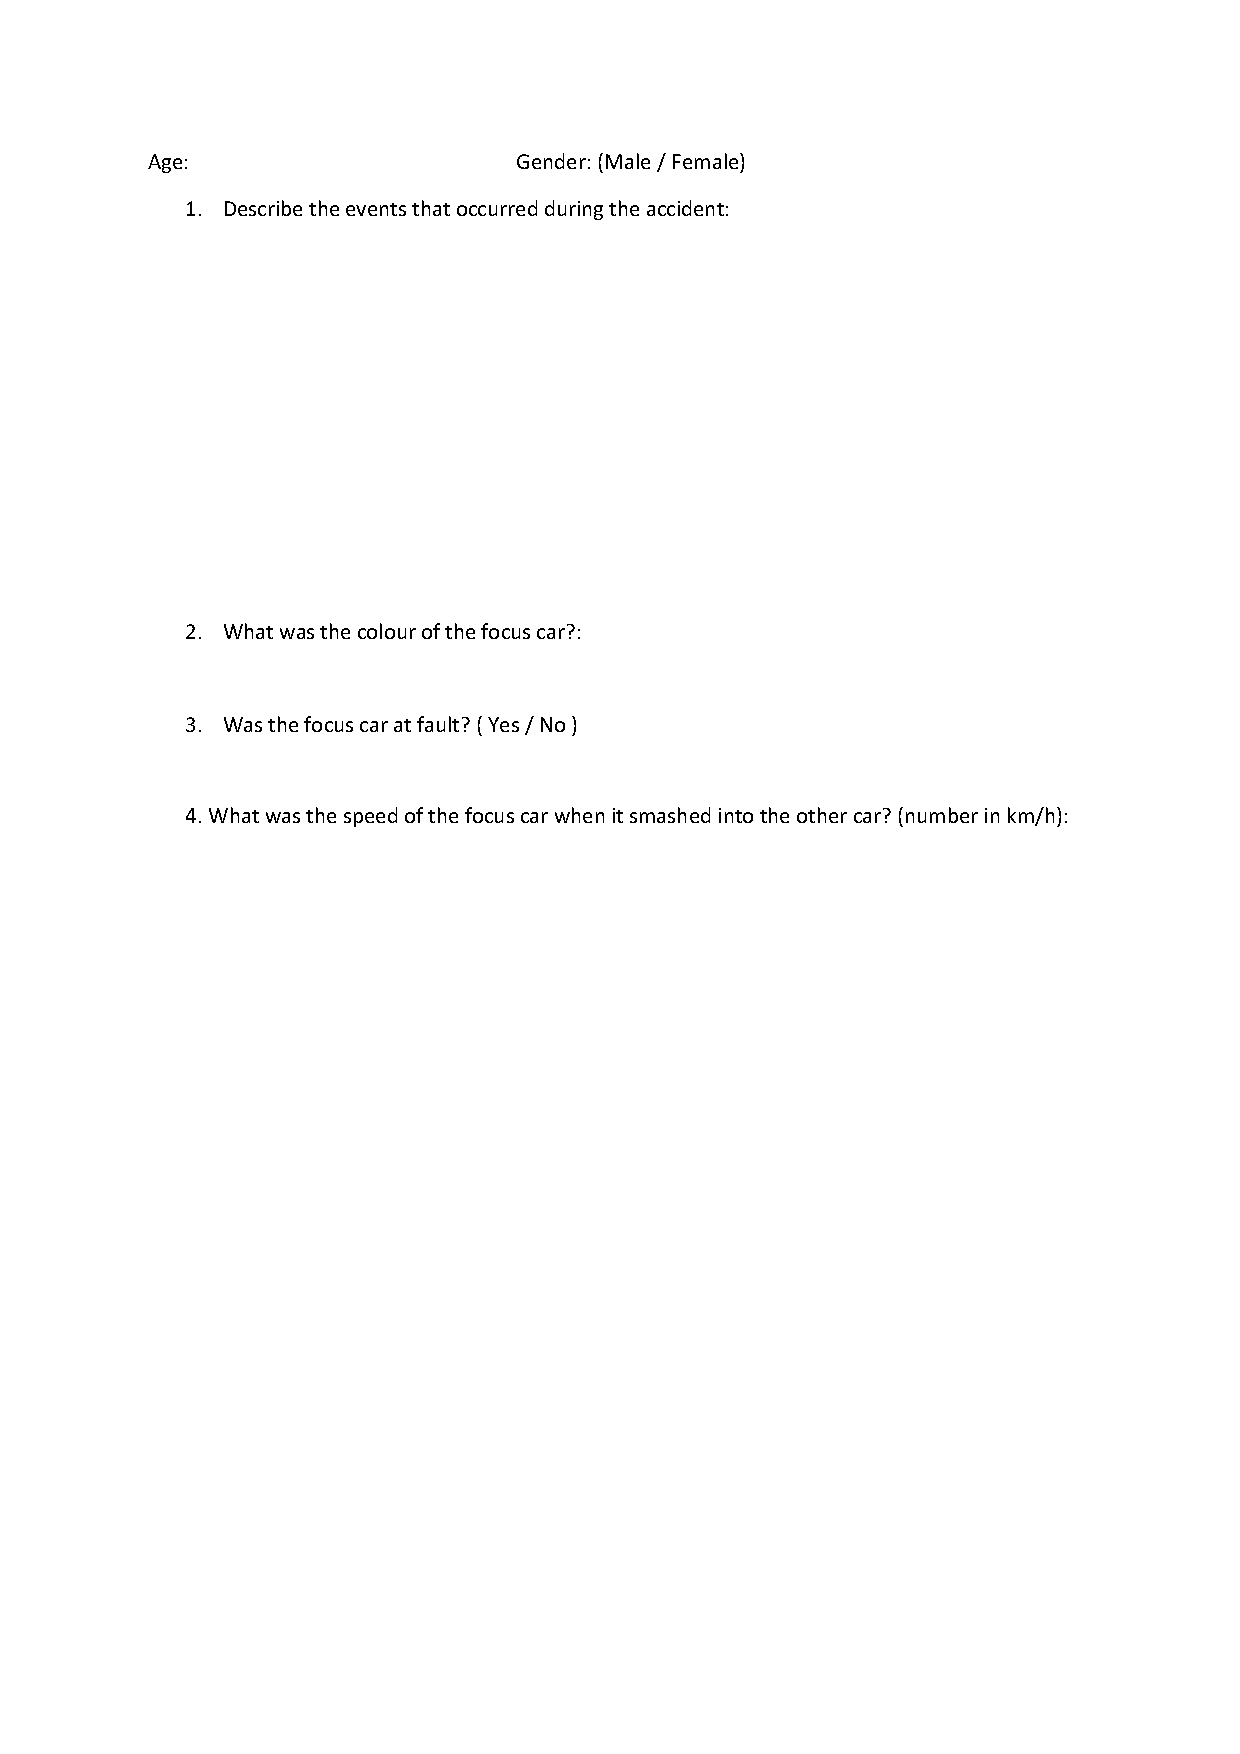
\includegraphics[width=\textwidth]{smashed.pdf}
~\label{ques:smashed}
\end{figure} 

\begin{figure}[H]
  \caption{ ~\\``Collided'' questionnaire} 
  \centering 
  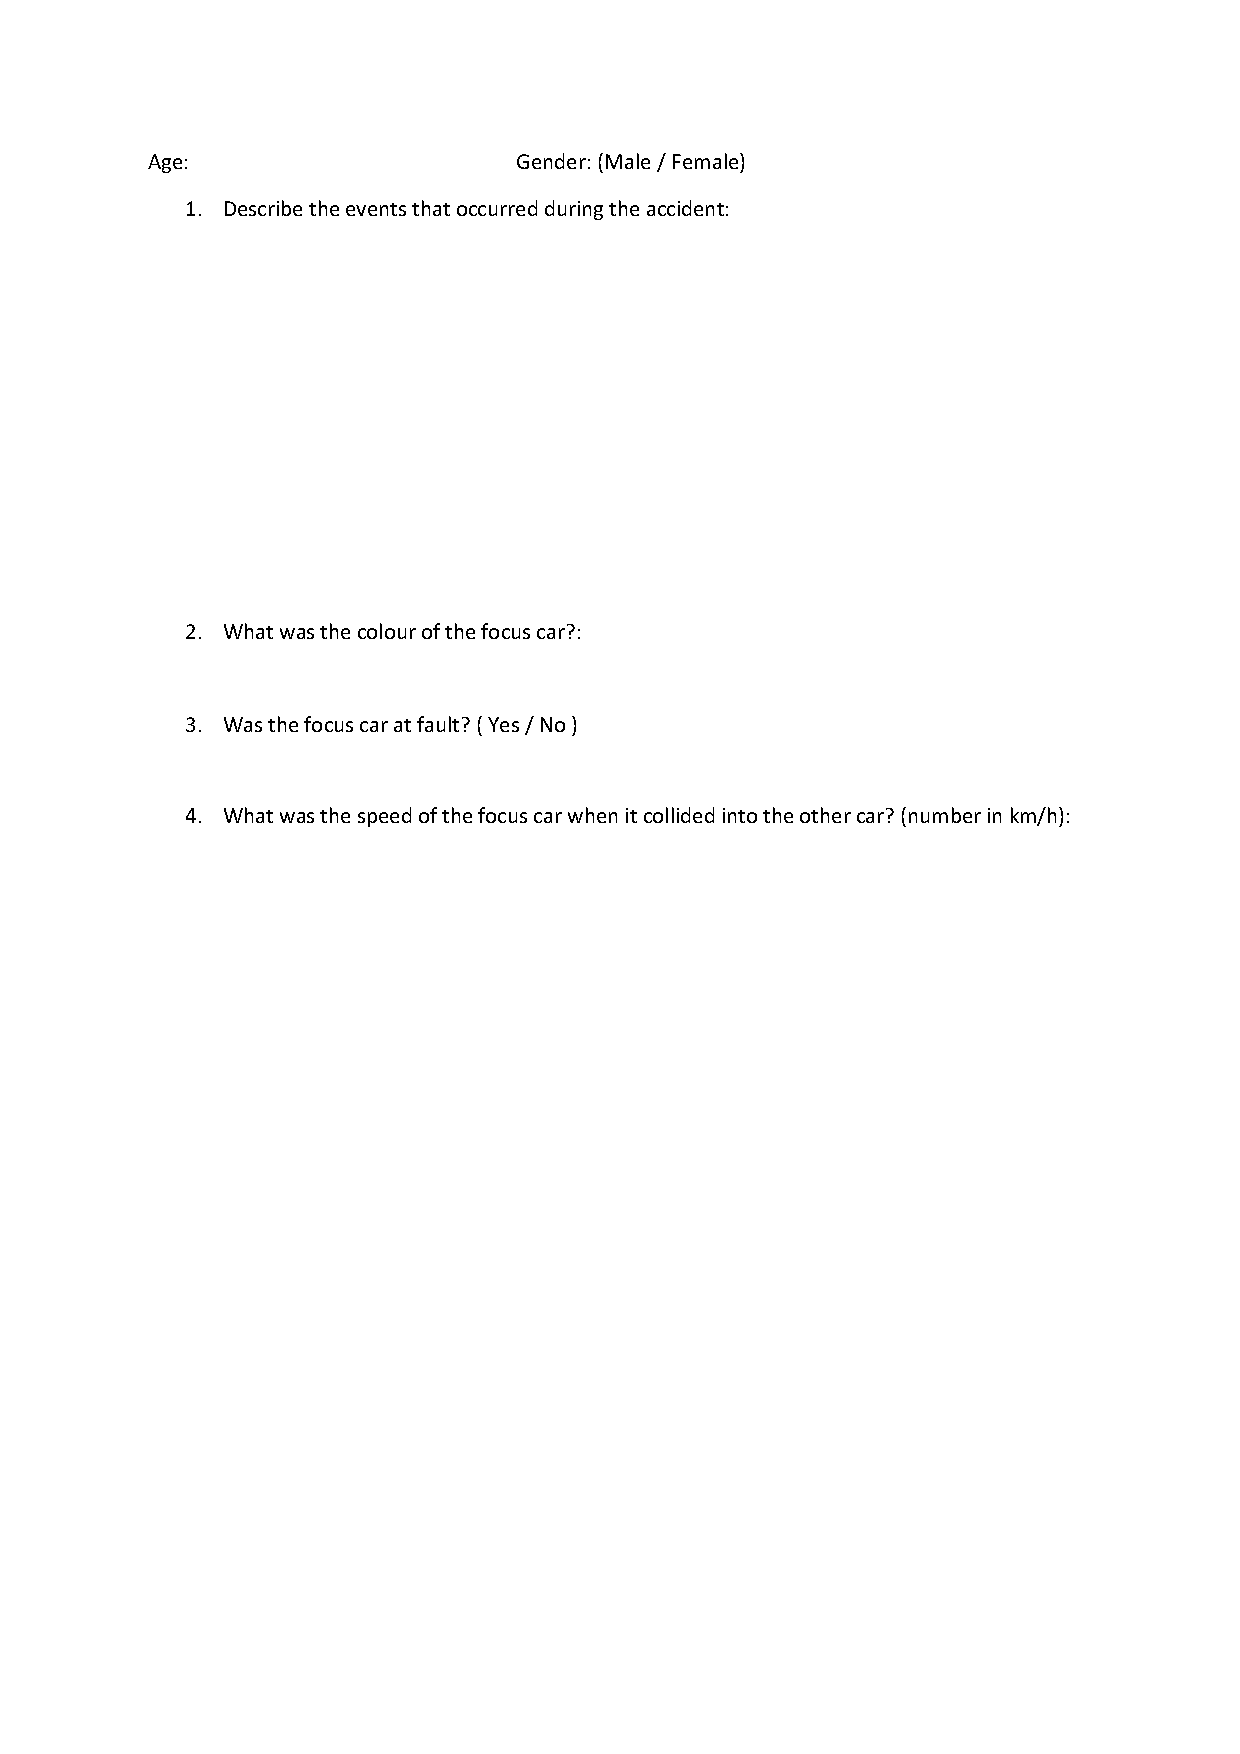
\includegraphics[width=\textwidth]{collided.pdf}
~\label{ques:collided}
\end{figure} 

\begin{figure}[H]
  \caption{ ~\\``Bumped'' questionnaire} 
  \centering 
  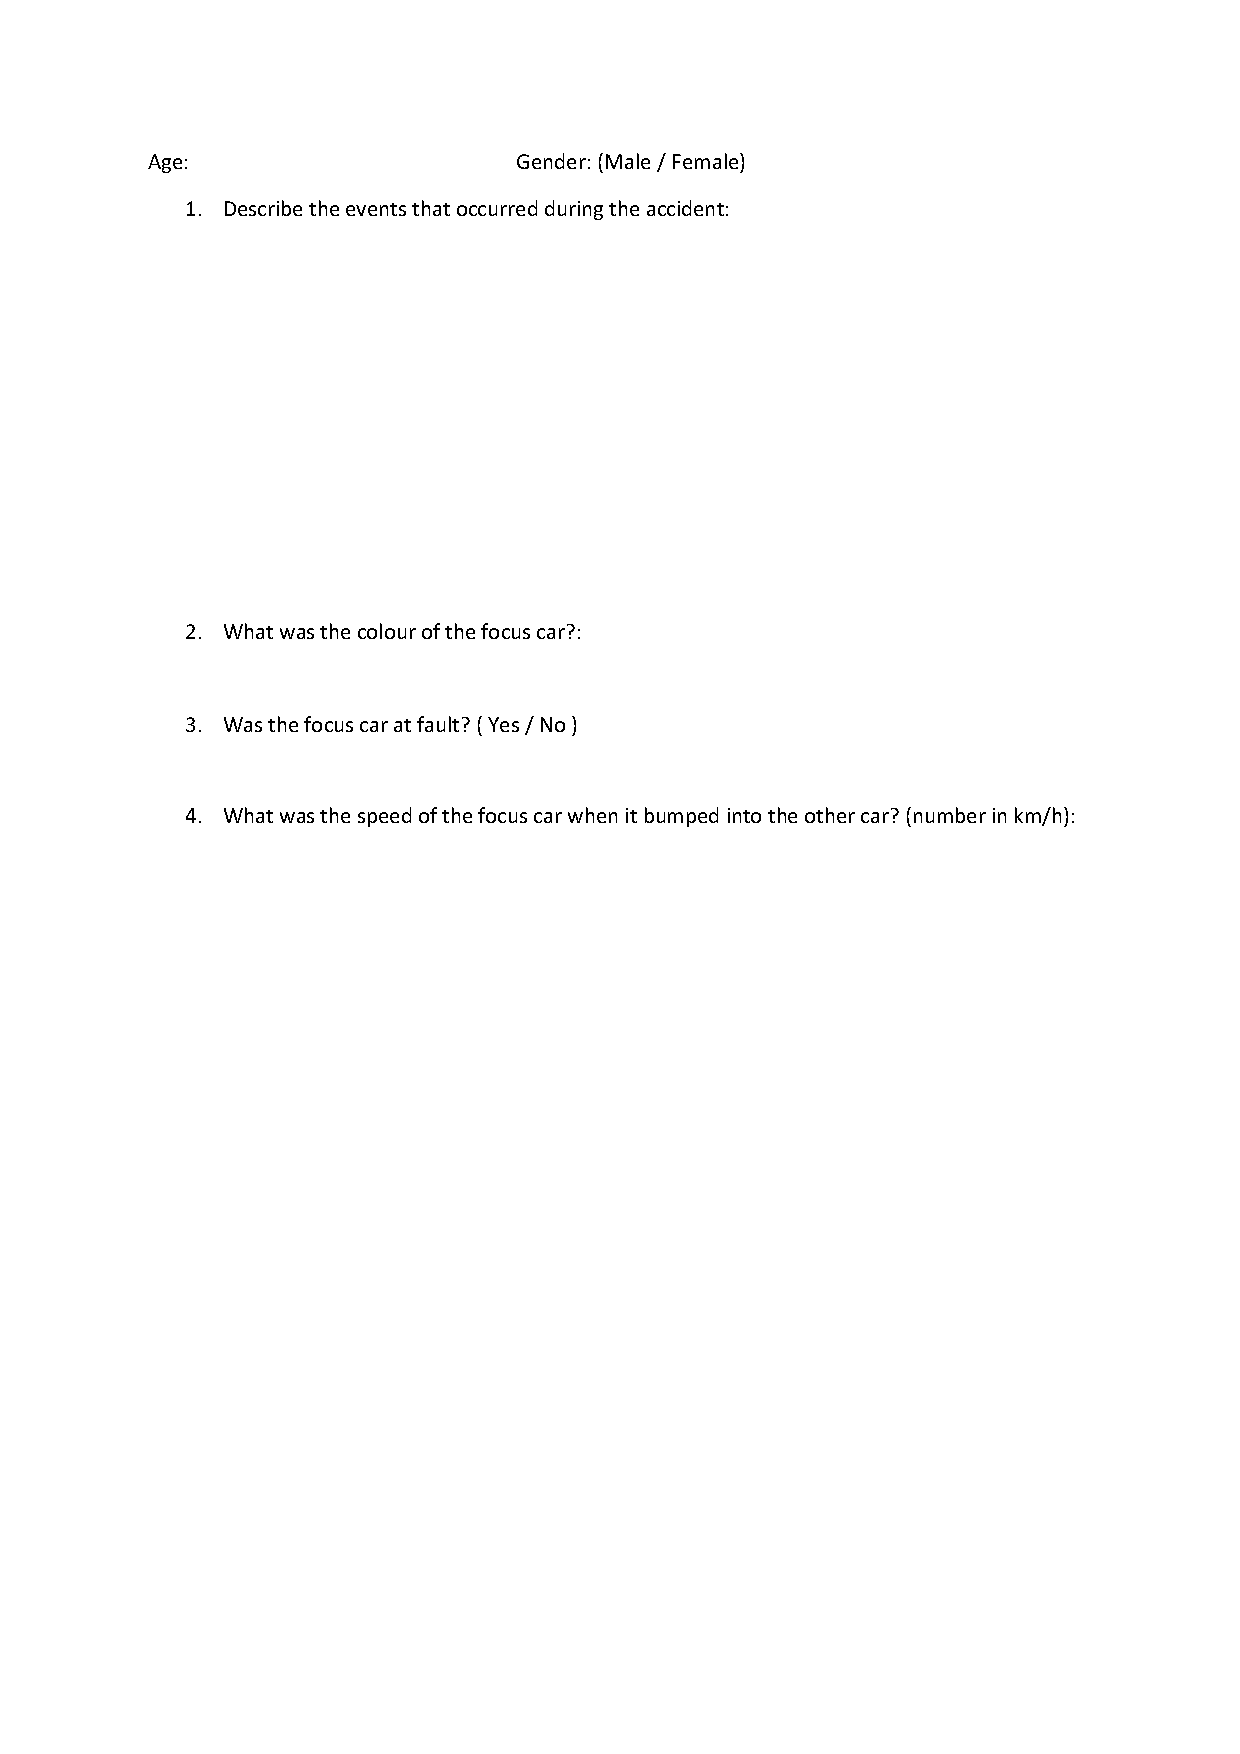
\includegraphics[width=\textwidth]{bumped.pdf}
~\label{ques:bumped}
\end{figure} 

\begin{figure}[H]
  \caption{ ~\\Briefing script} 
  \centering 
  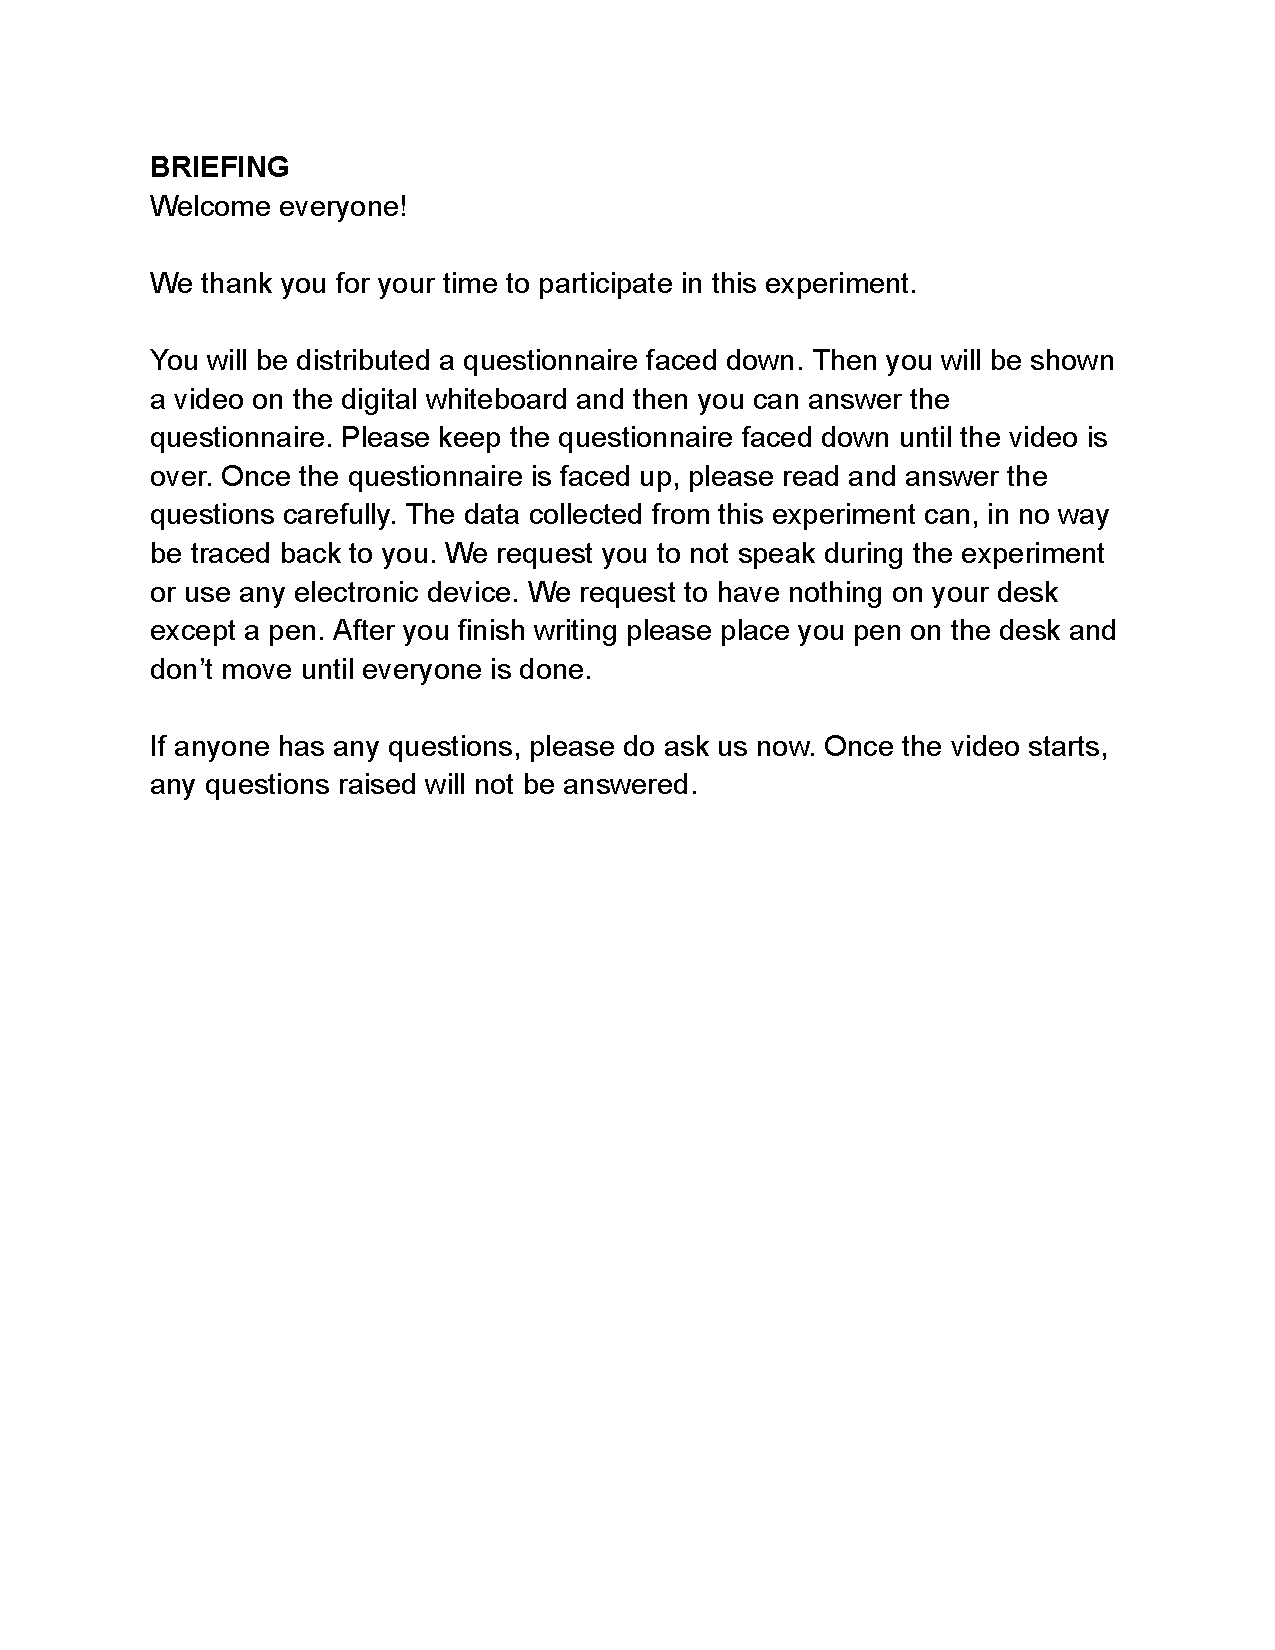
\includegraphics[width=\textwidth]{Briefing.pdf}
~\label{fig:briefing}
\end{figure} 

\begin{figure}[H]
  \caption{ ~\\Debriefing script} 
  \centering 
  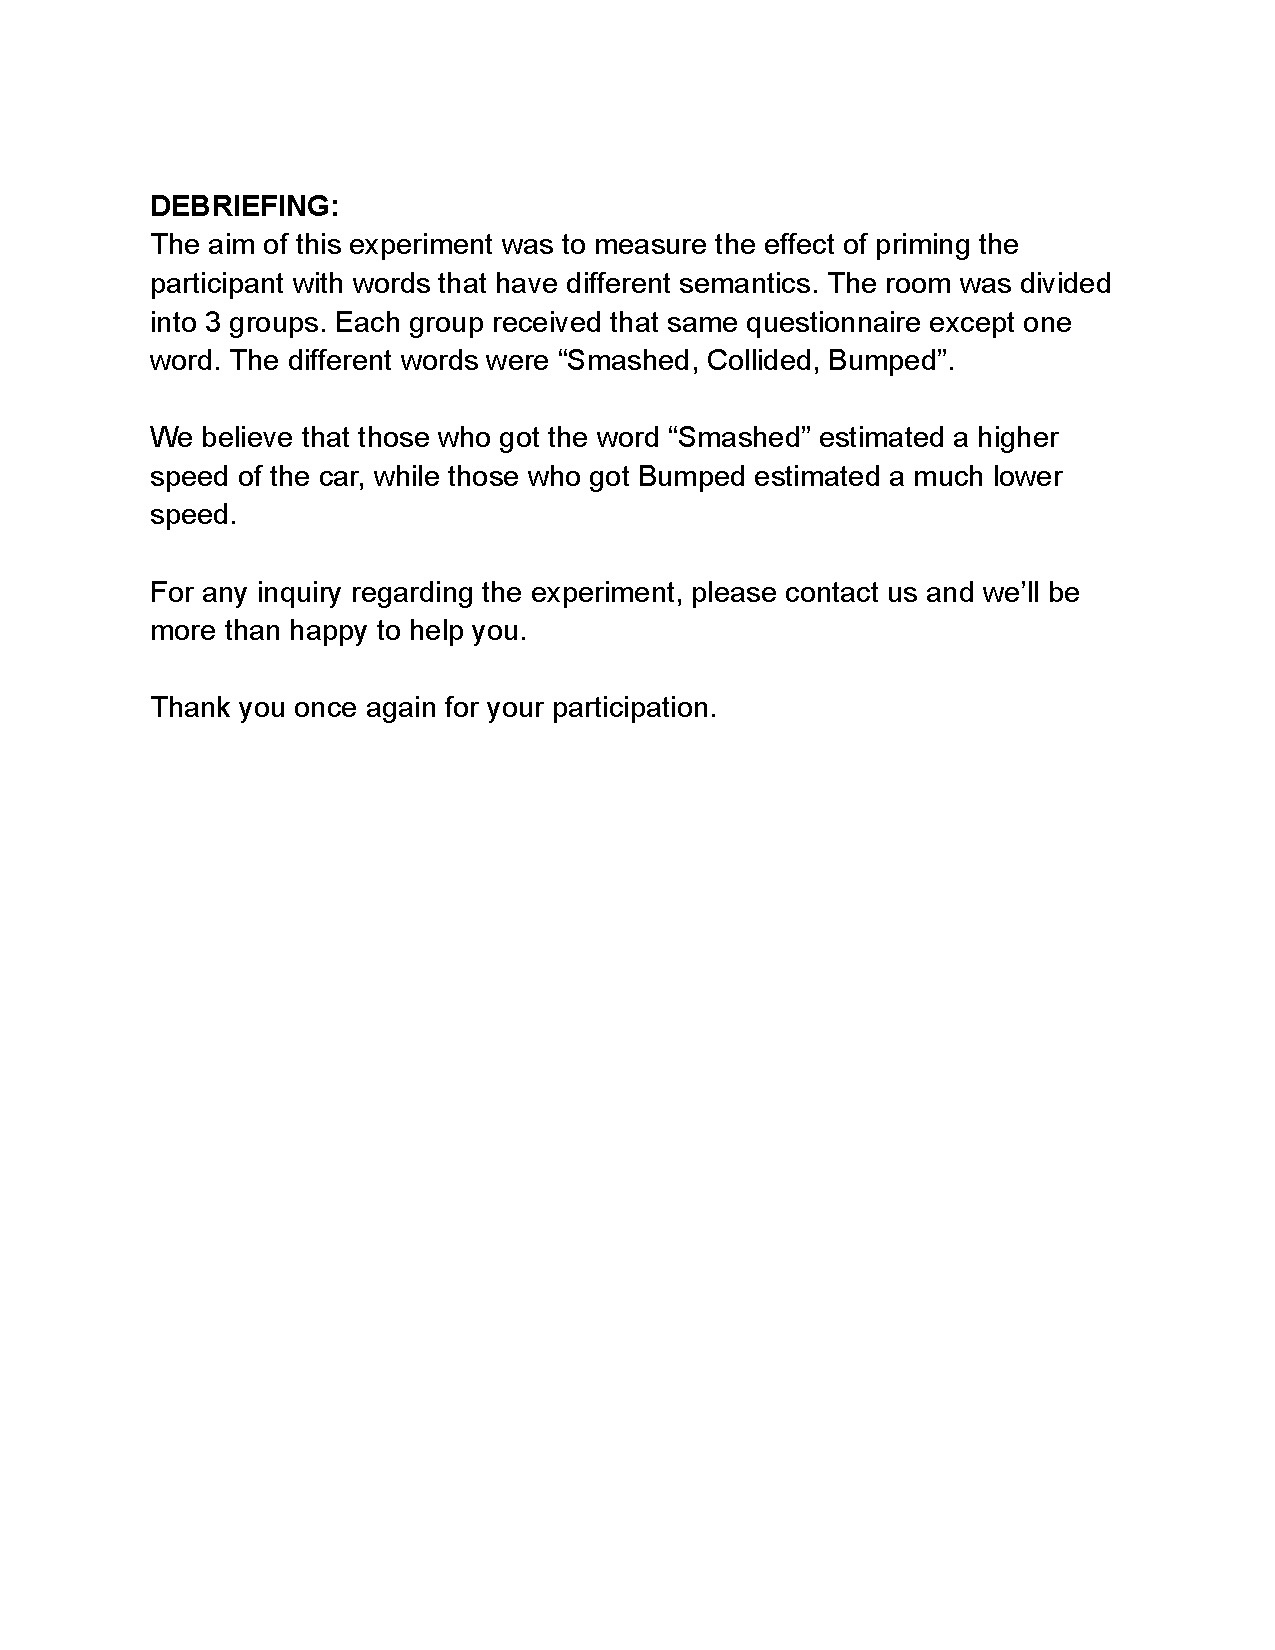
\includegraphics[width=\textwidth]{Debriefing.pdf}
~\label{fig:debriefing}
\end{figure} 

\begin{figure}[H]
  \caption{ ~\\Outlier Specimen} 
  \centering 
  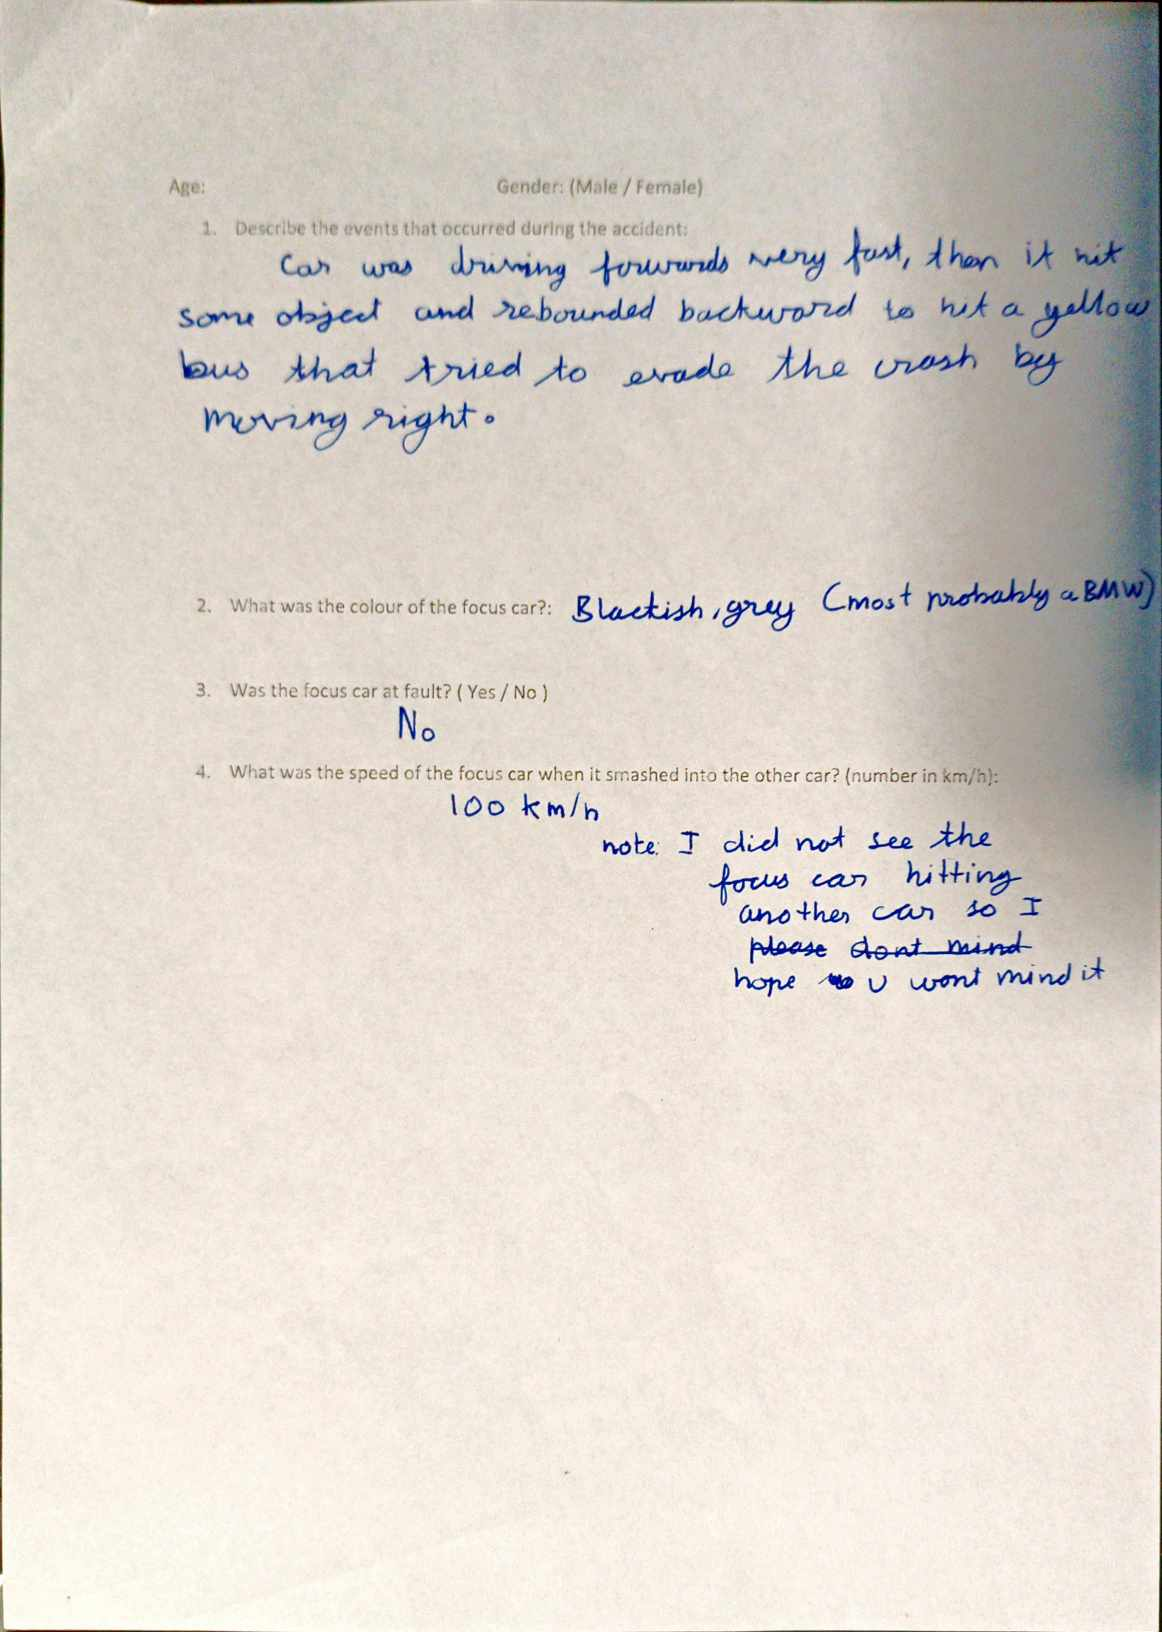
\includegraphics[width=\textwidth]{outlier.jpg}
~\label{fig:outlier}
\end{figure} 

\begin{figure}[H]
  \caption{ ~\\Jamovi Calculations} 
  \centering 
  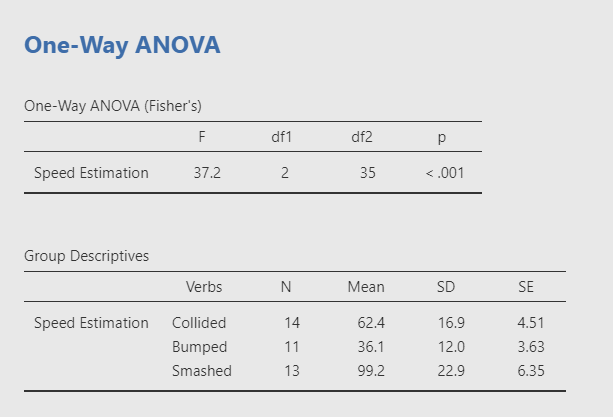
\includegraphics[width=\textwidth]{jamoviCalc.png}
~\label{fig:jamoviCalc}
\end{figure} 
\end{document}